\documentclass[memoire.tex]{subfiles}

\chapter{Analyse des solutions logicielles existantes}

Une fois nos critères définit, il faut décomposer le Big Data qui est un domaine très vaste, en plusieurs catégories~\cite{BIGDATA_OVERALL}. Une fois cette décomposition effectué, on va pouvoir s'intéresser aux outils existant permettant de réaliser chacune des tâches. On va noter leurs points faibles et leurs point forts ainsi que la manière dont ils sont censés être utilisés.

\section{Message Broker}

Un Message broker~\cite{MSG_BROKER}, Agent de message en français, est un moyen de communication utilisant des messages entre deux applications (Ex: Communication entre un serveur et un client). Un message broker permet une communication asynchrone entre applications. L'utilisation de cette solution permet de pouvoir facilement filtrer les messages que l'on reçoit et de stocker temporairement les messages reçus afin d'éviter les pertes de données. Ce dernier cas, s'avère très utile dans le cas où l'application chargée de la réception des données n'est pas en fonctionnement pendant un certains temps. Il existe deux types de communications avec un message broker : 

\subsubsection*{Publisher / Subscriber}

Dans ce mécanisme, l'entité envoyant les données est nommé "Publisher" et l'entité les récupérant est nommé "Subscriber". Le publisher va envoyer des données dans des topics \footnote{Un topic est une catégorie dans laquelle les messages produit sont stockés.} afin que les Subscribers de ce topic puissent les récupérer. Un publisher peut envoyer des données dans un ou plusieurs topics, et les subscribers peuvent être abonné à un ou plusieurs topics (Voir figure 2.1). 


\begin{figure}[!h]
	\centering 
	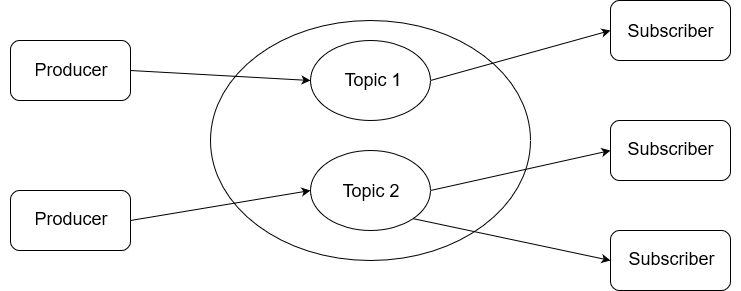
\includegraphics[scale=0.50]{img/producer_subscriber.png}
	\caption{Schéma du principe Producer/Subscriber}
	\label{Lambda}
\end{figure}

\subsubsection*{Point-to-point communication}

La communication point à point est la forme la plus simple de Producteur/Consommateur. Le producteur envoie ses données dans une queue et le consommateur va lire les messages dans la queue. Tout comme le modèle précédent, il peut y avoir plusieurs producteur et consommateurs sur la même queue, mais si plusieurs consommateurs sont présents, ils ne recevront des portions différentes des messages afin de favoriser le traitement concurrentiel.

\subsection{Kafka}

\subsection{ActiveMQ}

\subsection{RabbitMQ}

\section{Ingestion/Extraction de données}

La première catégorie, qui est aussi la première étape d'une architecture Big Data, c'est le récupération de données. Plus précisément comment nous allons récupérer des données, soit via des requêtes sur des sources externes, soit des sources externes nous envoie directement des données. 

\subsection{Apache Nifi}

\subsection{Talend}

\section{Traitement des données}

Une fois les données reçu, des traitements sont nécessaire afin de pouvoir stocker les données au format souhaité ou bien pour faire un tri des données utiles.

\subsection{Batch}

\subsubsection{Spark}

\subsubsection{Hadoop MapReduce}

\subsection{Streaming}

\subsubsection{Spark Streaming}

\subsubsection{Apache Storm}


\section{Stockage des données}

Une partie très importante du Big Data est le stockage des nombreuses données que l'ont reçoit. Il existe énormément de manières différentes de stocker des données selon la manière dont nous voulons les utiliser par la suite.

\subsection{Time Series}

\subsubsection{OpenTSDB}

\subsubsection{InfluxDB}

\subsection{Graph}

\subsubsection{Neo4j}

\subsubsection{JanusGraph}

\subsection{Clés/Valeurs}

\subsubsection{Redis}

\subsubsection{RoxDB}

\subsection{Documents}

\subsubsection{CouchDB}

\subsubsection{CouchBase}

\subsubsection{MongoDB}

\subsection{Wide Column}

\subsubsection{HBase}

\subsubsection{Cassandra}

\subsection{Système de fichiers}

\subsubsection{Hadoop HDFS}


\section{Visualisation et Analyse des données}

\subsection{Kibana}

\subsection{Banana}

\subsection{Grafana}

\subsection{Tableau}

\subsection{Click}